% Activate the following line by filling in the right side. If for example the name of the root file is Main.tex, write
% "...root = Main.tex" if the chapter file is in the same directory, and "...root = ../Main.tex" if the chapter is in a subdirectory.
 
%!TEX root =  

\chapter[MonteCarlo]{Monte Carlo}

In order to understand both the signal and backgrounds better, Monte Carlo (MC) datasets are computer-generated simulation events that allow a physicist to develop and validate an analysis.  The generation and refinement of MC algorithms and datasets could be a thesis in its own right, but this section will touch on some of the most relevant features of the MC datasets used in this algorithm.


\section{MC Creation Procedure}
\label{sec:mc-gen-overview}
MC events are generally created in four major steps.  
\begin{enumerate}
    \item First, the ``generator'' uses quantum field theory to simulate the hard scatter, generally starting with a proton and ending with all final-state particles.  
    \item Then those particles are handed off to a dedicated algorithm that simulates how they would shower and hadronize, where appropriate.  
    \item Next, the resulting particles from the first two steps are put into a detector simulation, which uses information on the detector materials and geometry to understand how the particles evolve as they travel through the ATLAS detector.  
    \item The detector's response to the particles is simulated in a digitization and reconstruction step, so that the final output is an event that looks similar to how a ``real'' event of that type might look in the ATLAS detector. 
\end{enumerate} 

\section{Signal Monte Carlo}
MadGraph \cite{MadGraph} is used to generate the signal MC, with showering and hadronization done in Pythia6 \cite{Pythia6}.  Madgraph uses a 5 flavor scheme PDF (parton distribution function), meaning that it models $b$-quarks in the proton as well as the more common light flavor (up, down, charm and strange quarks, and gluons).  In addition to the Higgs production with the associated $b$-quark and the Higgs decay, there can also be extra jets in the event from initial state radiation (ISR) and/or final state radiation (FSR).  We allow up to three additional partons per event in the signal MC; the generation and cross-section calculations tend to be more accurate for higher numbers of extra partons allowed but at the cost of exponentially slower and more complicated generation times.  We found three jets to be a reasonable cutoff where the distributions did not seem to be affected by allowing for higher numbers of extra partons, but the generation time was still acceptably quick.  

%--------------------------------------------------------
\begin{table}
   \caption{The signal MC samples and their parameters. \label{tab:sig_mc_parameters} }
    \begin{tabular}{ c c c }
    Dataset ID & mass (GeV) & width (GeV) \\
    181120     & 250        & 1.68682 \\
    181121     & 280        & 1.92318 \\
    181122     & 310        & 2.50849 \\
    181123     & 350        & 3.23507 \\
    181124     & 400        & 3.93561 \\
    181125     & 450        & 4.71906 \\
    181126     & 500        & 5.59454 \\
    181127     & 550        & 6.84368 \\
    181128     & 600        & 8.11044 \\
    181129     & 650        & 9.26688 \\
    181130     & 700        & 10.3760 \\
    181131     & 800        & 12.5049 \\
    \end{tabular}
\end{table}

%--------------------------------------------------------




The Madgraph signal generation is done for 12 different mass points, spanning 250-800 GeV. Below 250 GeV, the daughter $b$-jets from the Higgs tend to be too low-$p_T$ to fire the trigger, while above 800 GeV SUSY becomes less appealing theoretically.  Since both the production and decay of $bH\rightarrow bbb$ happen via SM interactions, with SUSY only becoming relevant for increasing the production cross section and widening the inherent width of the $A/H$ distributions, the signal generation can be done by using an SM $bH\rightarrow bbb$ production model but with a modified Higgs width.  There are 300,000 signal events generated for each mass point.

% ATF-II source: http://iopscience.iop.org/1742-6596/396/2/022031
The detector simulation for the signal MC was done using AtlFast-II (AFII) \cite{ATF2}, a modified version of Geant4 \cite{Geant4-1, Geant4-2} designed to cut down on the considerable time required for simulating particle interactions with the detector, especially showers in the calorimeter.  AFII does full simulation of the inner detector and tracking, but uses frozen shower shapes taken from a large collection of pre-generated samples to speed up the simulation.  After simulation, the digitization and reconstruction are handled by the ATLAS standard algorithms in the ATHENA framework, as is standard for all ATLAS MC.    

\section{Background}
\subsection{QCD Background}
Although QCD is the largest and most important background in this analysis, fully modeling it with QCD has some important drawbacks, which motivates our decision to use a mostly data-driven background estimation method.  That having been said, MC can still be a very valuable tool for making basic estimates and validating assumptions. 

There are two major types of QCD background in this analysis: first, when there is one or more mistakenly $b$-tagged light flavor or charm jets, which we call \textit{reducible} because, at least in theory, it could be identified and isolated/removed; and second, the \textit{irreducible} QCD background in which three real $b$-jets are present in the final state but without the intermediate resonance of the Higgs.  Both sources of background are expected to be significant but generally require different MC generation strategies.

\subsubsection{QCD Multijet}
The ATLAS QCD multijet MC collection is dataset is generated using Pythia8 \cite{Pythia8}.  One of the major challenges of a truly inclusive sample like this one is that low-$p_T$ jets dominate the production cross section but generally have very low efficiency through the triggers or analysis cut flows, which is addressed by generating events several times with filtering applied based on the $p_T$ of the leading jet.  This leads to a distinctive ``slice'' structure to the sample, where 8 different slices are generated, each with a different $p_T$ range for the leading jet, and then the slices are knitted together with different relative weights to produce an inclusive spectrum with high statistics at all $p_T$ values.  


ATLAS has a high-statistics inclusive QCD MC sample that is used primarily in this analysis for understanding the QCD background from mistagged charm and light flavor.  Since the sample is inclusive, there is no filtering on the flavor of the jets that are produced (although there is dedicated effort to have high-$p_T$ jets simulated with adequate statistics) and the vast majority of jets are light or charm jets.  As a result, while we use this sample to estimate the efficiency and flavor composition of the QCD production in ATLAS as a whole, a particularly important background (QCD $bbb$) is virtually absent from this sample.


\subsubsection{$b$-Enriched QCD Multijet}
Since the inclusive QCD Multijet samples are inadequate for understanding the $bb$ and $bbb$ MC backgrounds, we generate a dedicated sample that undergoes filtering to enrich it in heavy flavor.  This sample is generated using Sherpa 1.4.3 \cite{Sherpa} and detector simulation is done with AFII.  This sample starts with a 5-flavor PDF that assumes massive $b$-quarks and 2, 3 or 4 final state partons; then a filter is applied that requires that the leading 2 partons in the event be true $b$-quarks as well as requiring that the leading parton have a $p_T$ of at least 55 GeV (the latter requirement helps keep an acceptable efficiency when the sample is passed through the trigger and offline cuts).
i

%---------------------------------------
\begin{table}[h]
 \begin{center}
    \begin{tabular}{l|r}
   subprocess      & cross section (pb)\cr \hline

$jj\rightarrow b\bar{b}jj$ & 58531 \cr
$jj\rightarrow b\bar{b}j$ & 33411 \cr
$bj\rightarrow bjj \ \ +\ \  \bar{b}j\rightarrow \bar{b}jj$ & 22147 \cr
$bj\rightarrow bjjj \ \ +\ \  \bar{b}j\rightarrow \bar{b}jjj$ & 16282 \cr
$bj\rightarrow b j \ \ +\ \  \bar{b} j\rightarrow \bar{b} j$ & 12135 \cr
$jj\rightarrow b\bar{b}$ &  1672 \cr
$cj\rightarrow c b\bar{b}j \ \ +\ \  \bar{c} j\rightarrow \bar{c}  b\bar{b}j$ & 1602 \cr
$bj\rightarrow b b\bar{b}j \ \ +\ \  \bar{b} j\rightarrow \bar{b}  b\bar{b}j$ & 997 \cr
$jj\rightarrow b\bar{b}c\bar{c}$ &  776 \cr
$cj\rightarrow c b\bar{b} \ \ +\ \  \bar{c} j\rightarrow \bar{c}  b\bar{b}$ & 681 \cr
$bj\rightarrow b b\bar{b} \ \ +\ \  \bar{b} j\rightarrow \bar{b}  b\bar{b}$ & 387 \cr
$jj\rightarrow b\bar{b}b\bar{b}$ &  376 \cr
$b\bar{c}\rightarrow b\bar{c}j \ \ +\ \  \bar{b} c\rightarrow \bar{b} cj$ & 206 \cr
$bc\rightarrow bcj\ \ +\ \  \bar{b}\bar{c}\rightarrow \bar{b} \bar{c}j$ & 194 \cr
$b\bar{c}\rightarrow b\bar{c}jj \ \ +\ \  \bar{b} c\rightarrow \bar{b} cjj$ & 143 \cr
$bc\rightarrow bcjj\ \ +\ \  \bar{b}\bar{c}\rightarrow \bar{b} \bar{c}jj$ & 136 \cr
$bc\rightarrow bc\ \ +\ \ \bar{b}\bar{c}\rightarrow \bar{b} \bar{c}$ & 122 \cr
$b\bar{c}\rightarrow b\bar{c} \ \ +\ \  \bar{b} c\rightarrow \bar{b} c$ & 121 \cr
$b\bar{b}\rightarrow b\bar{b}j$ & 62 \cr
$bb\rightarrow bbj\ \ +\ \  \bar{b}\bar{b}\rightarrow \bar{b} \bar{b}j$ & 53 \cr
$b\bar{b}\rightarrow b\bar{b}jj$ & 44 \cr
$bb\rightarrow bbjj\ \ +\ \  \bar{b}\bar{b}\rightarrow \bar{b} \bar{b}jj$ & 39 \cr
$b\bar{b}\rightarrow b\bar{b}$ & 37 \cr
$bb\rightarrow bb\ \ +\ \  \bar{b}\bar{b}\rightarrow \bar{b} \bar{b}$ & 30 \cr
\hline
   \end{tabular}
\caption{Hard subprocesses simulated in the bb QCD MC event sample, along with their cross sections. Here
$j=u,\bar{u},d,\bar{d},s,\bar{s},g$}
\label{tab:sherpa_subprocesses}
  \end{center}
\end{table}
%---------------------------------------



%-----------------------------------------------                     
\begin{figure}
  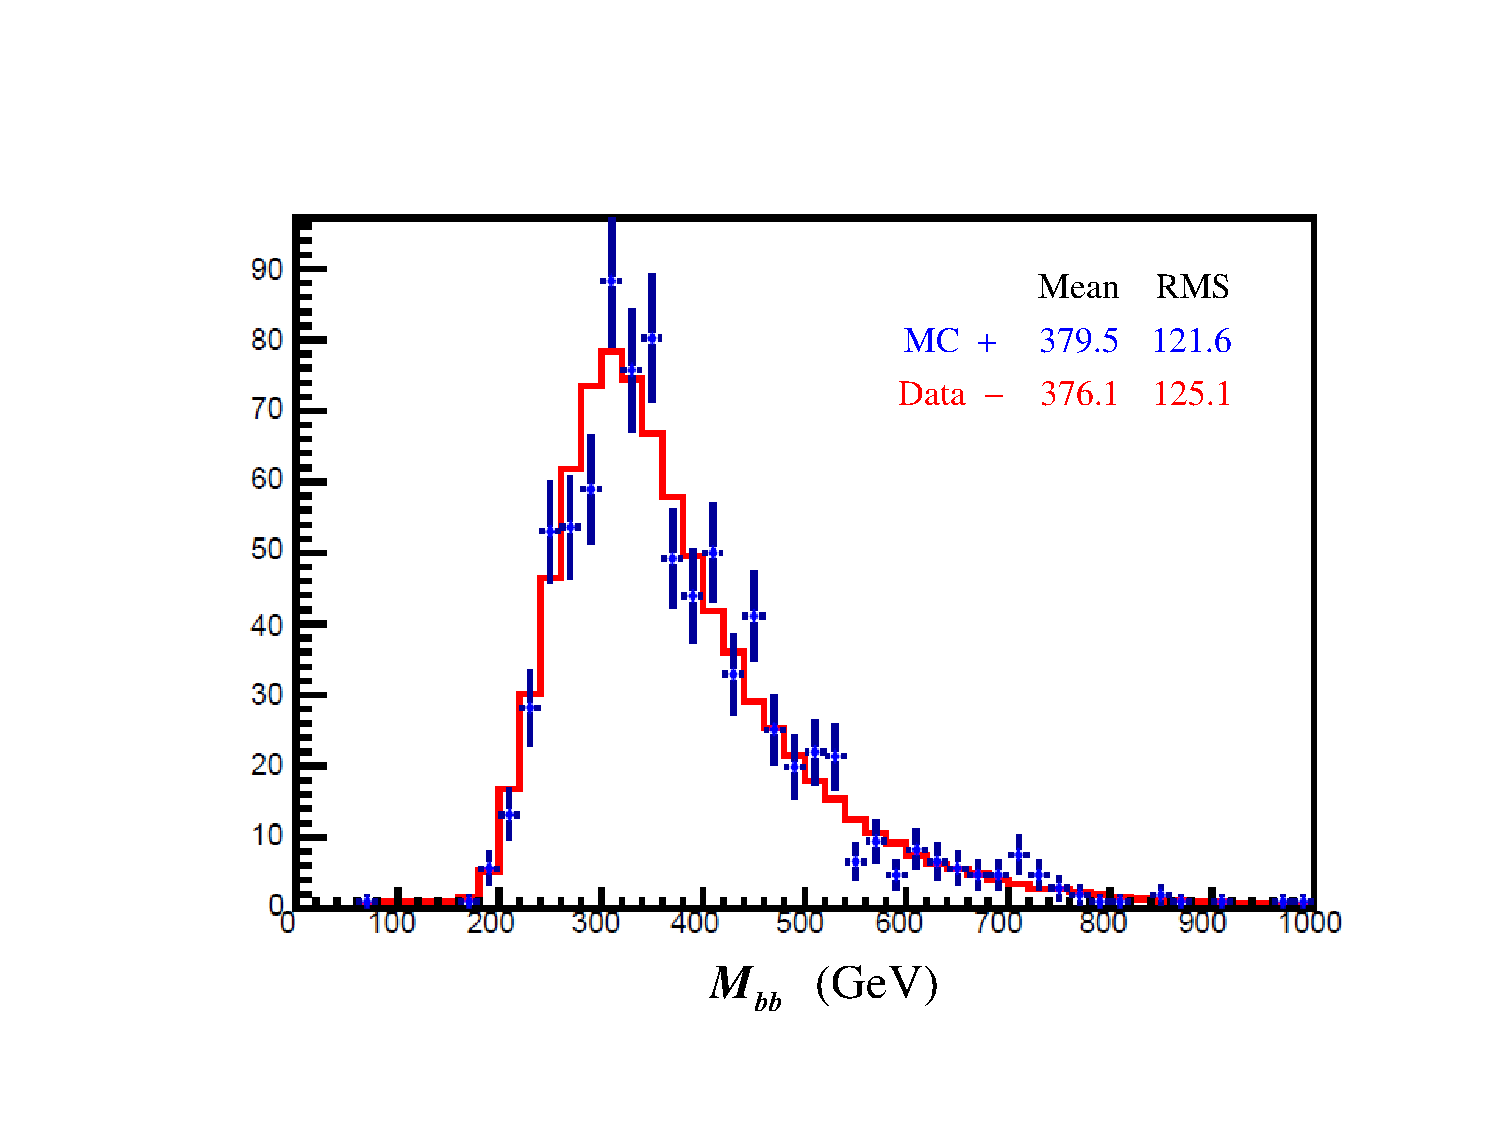
\includegraphics[width=0.70\linewidth]{MonteCarlo/figures/mbb_bbqcd_vs_data.pdf}
  \caption{Mass of the two leading jets in events passing all cuts except the
bbb, bbloose and bbanti classification.  Distributions for the 10,000 event bb QCD Monte Carlo validation sample
and a 2.2~fb$^{-1}$ luminosity data sample are shown.    \label{fig:mbb_bbqcd_vs_data}}
\end{figure}

\begin{figure}
  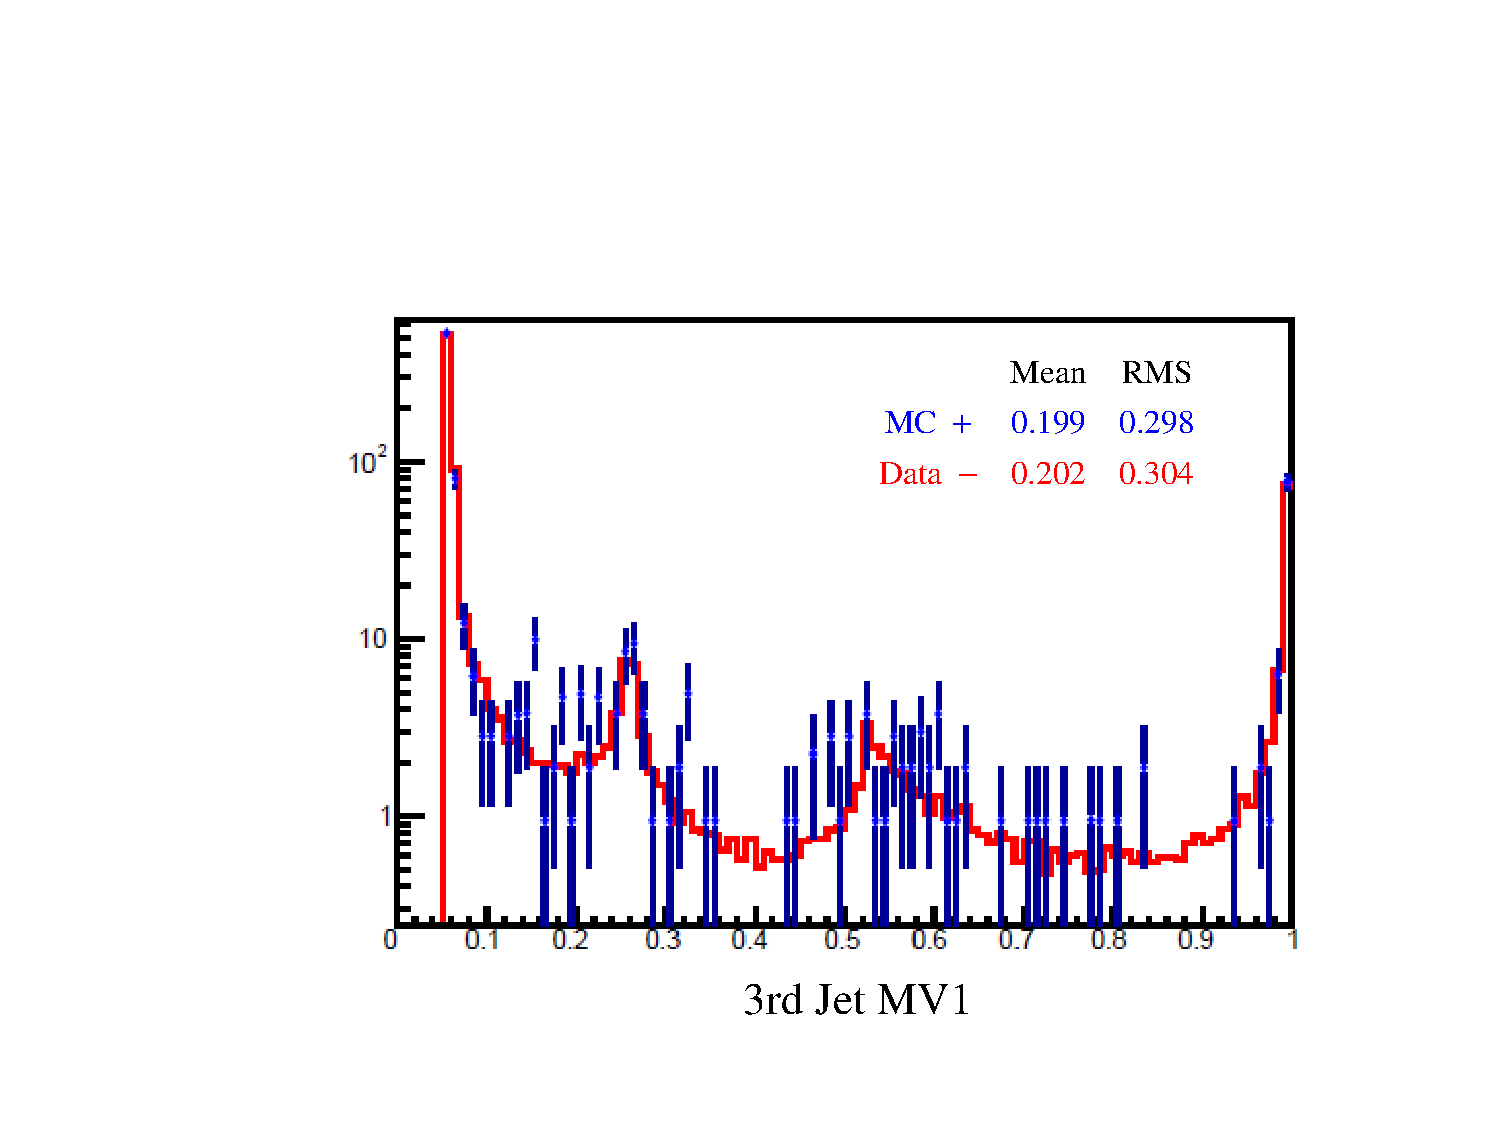
\includegraphics[width=0.70\linewidth]{MonteCarlo/figures/mv1_jet3_bbqcd_vs_data.pdf}
  \caption{The b-tag variable MV1 for the 3rd leading $p_T$ jet in events passing all cuts except the
bbb, bbloose and bbanti classification.     Distributions for the 10,000 event bb QCD Monte Carlo validation sample
and a 2.2~fb$^{-1}$ luminosity data sample are shown.    \label{fig:mv1_jet3_bbqcd_vs_data}}
\end{figure}




\begin{figure}
  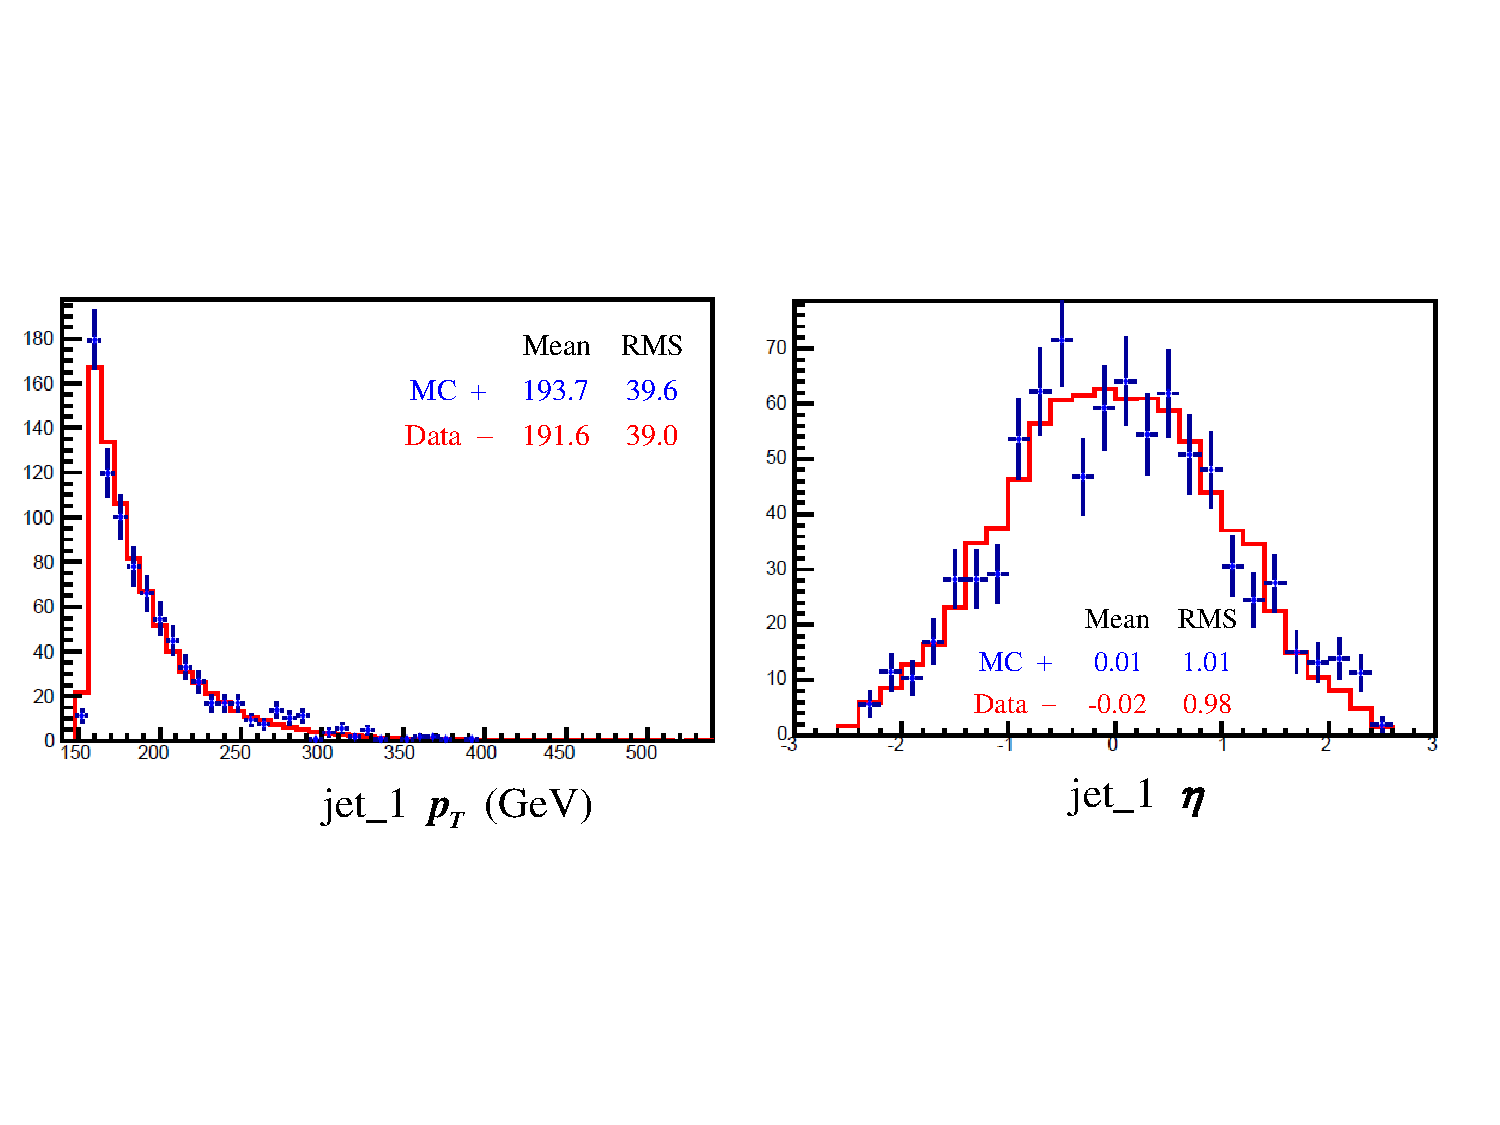
\includegraphics[width=0.85\linewidth]{MonteCarlo/figures/pt_eta_jet1_bbqcd_vs_data.pdf}
  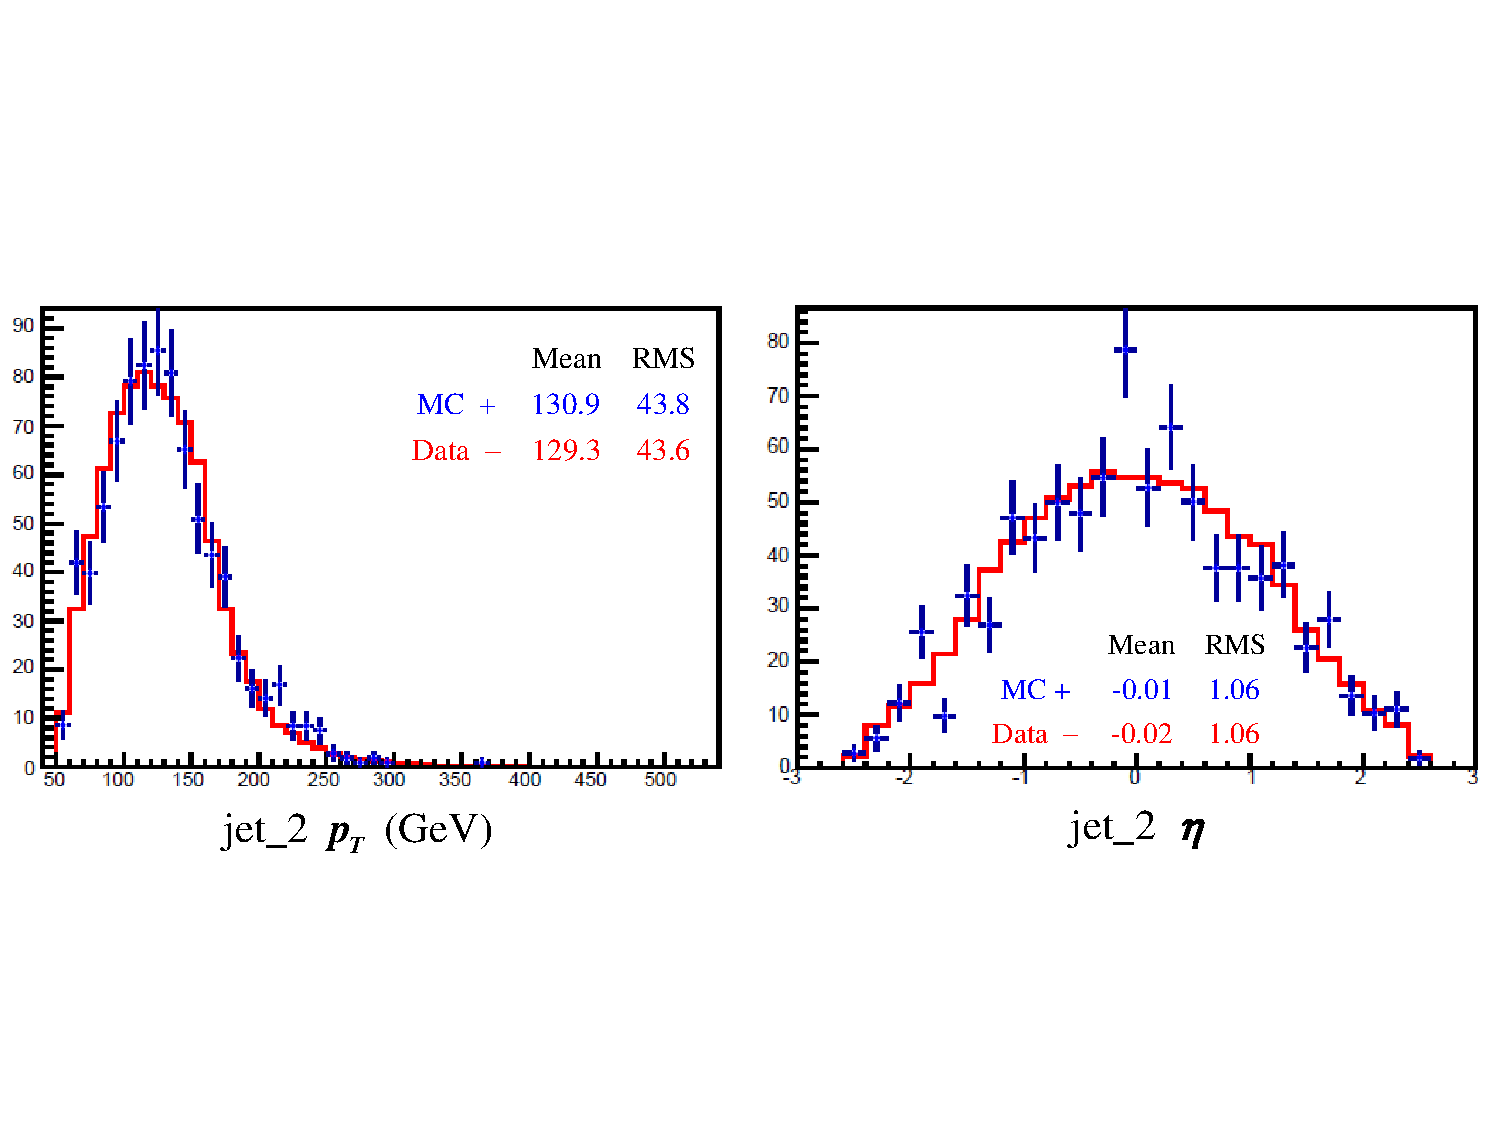
\includegraphics[width=0.85\linewidth]{MonteCarlo/figures/pt_eta_jet2_bbqcd_vs_data.pdf}
  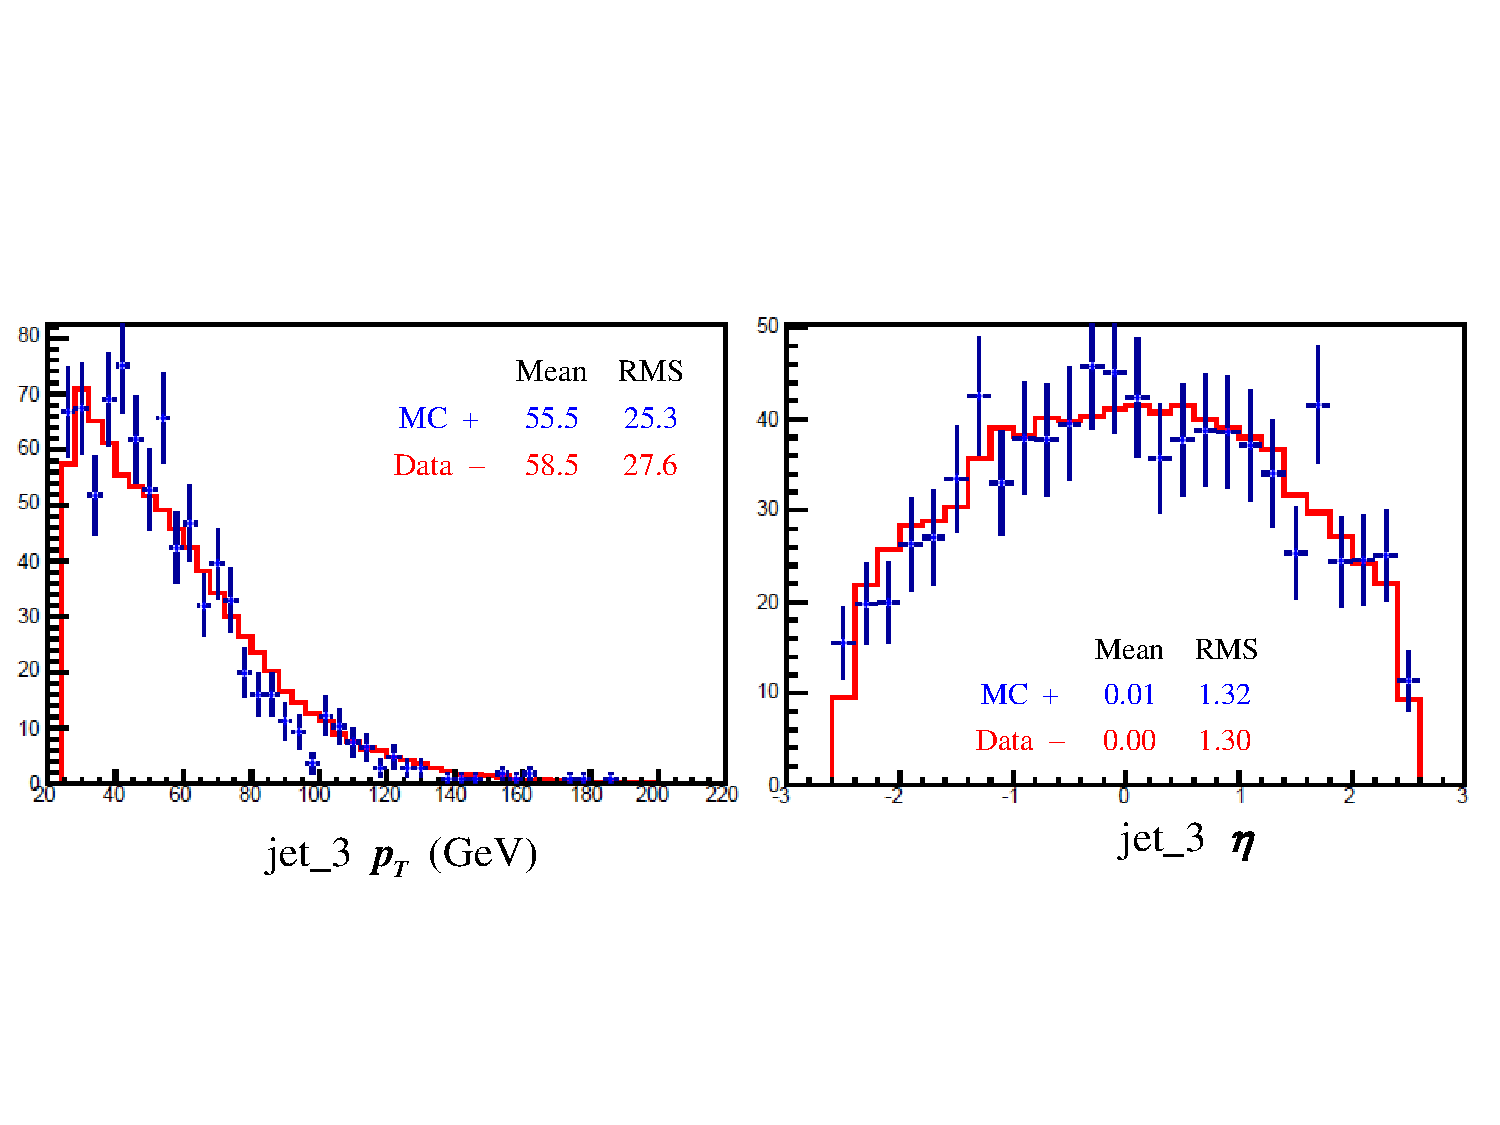
\includegraphics[width=0.85\linewidth]{MonteCarlo/figures/pt_eta_jet3_bbqcd_vs_data.pdf}
  \caption{$p_T$ and $\eta$ for the three leading $p_T$ jets in events passing all cuts except the
bbb, bbloose and bbanti classification.     Distributions for the 10,000 event bb QCD Monte Carlo validation sample                 
and a 2.2~fb$^{-1}$ luminosity data sample are shown.    \label{fig:pt_eta_bbqcd_vs_data}}                                          
\end{figure}                                                                                                                        
%-----------------------------------------------                     



\subsection{Top Background}











